\documentclass{article}
\usepackage[utf8]{inputenc}
\usepackage{graphicx}
\graphicspath{ {./images/} }
\usepackage[rightcaption]{sidecap}

\title{}
\date{}


\begin{document}
\maketitle
\begin{center}
\textbf{Universidade Federal Fluminense - uff}

\textbf{Escola de Engenharia – TCE }

\textbf{Departamento de Engenharia de Telecomunicações - TET }

\textbf{Grupo PET do Curso de Engenharia de Telecomunicações - PET-Tele }
\vfill
\textbf{\huge Sistema para armazenamento, compartilhamento e versionamento de software}

\vfill
\textbf{\Large João Guilherme Coutinho Beltrão }
\vfill
\textbf{entregue em: 03/04/2021}

\textbf{ data limite: 04/04/2021}
\vfill
\newpage
\end{center}


\section{Objetivo}

\hspace{4mm} O objetivo a ser alcançado com esse projeto é mostrar o uso de sistemas para armazenamento, compartilhamento e versionamento de software, em especial o sistema \textit{Git}. Assim como sua história e importância, visando o uso em projetos do grupo PET. Além disso, também será estudado ambientes de hospedagem de código como o \textit{GitHub} e o \textit{GitLab}.

\section{Motivações}
\begin{itemize}
    \item Aprender e aprofundar o conhecimento sobre o sistema de versionamento \textit{Git}.
    \item Implementar o uso de software como o \textit{Git}, em projetos do grupo PET, para facilitar o versionamento e construção de códigos em grupo.
    \item Implementar também o uso de ambientes de hospedagem como \textit{GitHub} e \textit{GitLab} para otimizar o compartilhamento e armazenamento de códigos de um projeto.
\end{itemize}

\section{Versionamento}
\subsection{O que é versionamento?}
\hspace{4mm} Versionamento de software é o processo de salvar momentos de um documento para que esses possam ser acessados no futuro caso erros ou mudanças indesejáveis ocorram. Dessa forma o usuário consegue ter acesso a vários estados do projeto prevenindo-se contra problemas com o mais recente. 

Porém, versionar um projeto manualmente tem muitas desvantagens. \\Primeiramente, é muito trabalhoso para salvar todos os estados de um código, logo, algumas versões se perdem, o que não é o ideal. Outro problema é quando se trabalha com mais pessoas, já que cada pessoa estaria salvando seu próprio código podendo conflitar no momento da união. Para resolver esse problemas foram criados os softwares de controle de versão (GUANABARA, 2020).

\subsection{Software de controle de versão}
\hspace{4mm}Os softwares de controle de versão (também chamados de SVC) são softwares que auxiliam o programador a fazer o versionamento de seu projeto. Neles cada pequena mudança do código será salva, sem o risco de perder o arquivo, além de facilitar o processo de armazenamento e compartilhamento dos arquivos. Foram criados dois tipos de software de controle de versão: centralizado e distribuído.

\subsubsection{SVC centralizado}
\hspace{4mm}Nos SVC centralizados quando o programador vai salvar um estado do código, o SVC mandará o arquivo para um repositório local conectado ao mesmo servidor que o computador está usando. Dessa forma, um grupo de programadores trabalhando no mesmo projeto, conseguirão salvar todos os arquivos em um único lugar e compará-los, além de acessarem todas as versões anteriores desses arquivos. A desvantagem desse tipo de versionamento é a dependência ao servidor do repositório. É necessário estar conectado constantemente para acessar os arquivos ou criar arquivos novos. Na versão do SVC distribuído já não apresenta esse problema.

\subsubsection{SVC distribuído}
\hspace{4mm}Nos SVC distribuídos, o salvamento do estado do código pelo programador pode ser feito em um repositório local dentro do próprio computador.

Posteriormente, esse arquivo será direcionado a um repositório remoto onde será feito o armazenamento de todos os documentos e assim sendo facilmente acessado pelo grupo de programadores.

\subsubsection{Vantagens de um SVC}
\begin{itemize}
    \item O programador tem total controle e fácil acesso a todas as versões anteriores de seu código e quais são as diferenças de cada versão.
    \item A equipe de programadores consegue se ramificar e facilmente juntar os códigos no final do projeto.
    \item Auxilia na organização do projeto como um todo.
\end{itemize}

\section{\textit{Git}}
\hspace{4mm}\textit{Git} é um software de controle de versão distribuído criado em 2005 por Linus Torvalds (criador do sistema operacional Linux) e é atualmente o SVC mais usado no mercado. Ele ficou popular por alguns motivos:
\begin{itemize}
    \item É Open Source, diferente de seu principal concorrente da época (BitKeeper). 
    \item Possui uma performance muito superior aos outros SVC da época.
    \item É distribuído, o que é incontestavelmente melhor do que os SVC centralizados.
\end{itemize}
\subsection{Repositório remoto}
\hspace{4mm}Antes de começar a usar o \textit{Git} para versionar seus projetos, é preciso entender o que são os repositórios remotos. Como já foi dito, os SVC distribuídos versionam os códigos mandando-os primeiramente para um repositório local e em seguida para o remoto. Nesse caso, o \textit{Git} desempenha o papel do repositório local, porém para o remoto precisamos usar outra plataforma. As principais plataformas que funcionam como repositório remoto são o \textit{GitHub} e o \textit{GitLab}.
\subsubsection{\textit{GitHub} vs \textit{GitLab}}
\hspace{4mm}\textit{Github} e \textit{Gitlab} são plataformas de hospedagem de código-fonte. Elas permitem que os desenvolvedores contribuam em projetos privados ou abertos, e ambas fazem o controle de versão dos projetos hospedados utilizando o \textit{Git} (BERTOLA, 2019).

A principal diferença entre elas é que o \textit{GitLab} foca na integração. Além de proporcionar, nativamente, ferramentas de integração e entrega contínua. Já o \textit{GitHub} foca em eficácia e desempenho de infraestrutura, e assim se configura como a melhor opção para projetos com muitos programadores. 
\subsection{Como usar o \textit{Git}}
\hspace{4mm}O \textit{Git} por ser um software Open Source, é totalmente gratuito. Para baixa-lo, basta entrar no site \textit{git-scm.com} e iniciar o download. Além disso para usá-lo com maior eficácia é importante criar uma conta nas plataformas de hospedagem, como o \textit{GitHub}.

\subsubsection{Usando Git pelo terminal}
\hspace{4mm}Com o \textit{Git} instalado podemos começar a usá-lo. Para isso, alguns comando do \textit{Git} são necessários.
\begin{enumerate}
    \item HELP
    
    \hspace{4mm}Esse é o primeiro comando importante que se deve conhecer, com ele o programador é mandado para páginas de tutorial sobre cada um dos outros comandos.
    
    \textit{git help "comando"}
    \item INIT
    
    \hspace{4MM}Esse comando cria um repositório local no arquivo que estiver sendo acessado no momento. 
    
    \textit{git init}
    \item STATUS
    
    \hspace{4mm}Esse comando mostra se ocorreu alguma alteração no repositório e o que pode se fazer com elas. 
    
    \textit{git status}
    \item ADD
    
    \hspace{4mm}Com esse comando o programador passa uma das modificações mostradas pelo status para a fila de commits.
    
    \textit{git add "nome do arquivo"}
    \item COMMIT
    
    \hspace{4mm}Esse comando faz o \textit{"commit"} das mudanças na fila de \textit{commits}, ou seja, mandá-los para o repositório local.
    
    \textit{git commit -m "comentario sobre a mudança"}
    \item PUSH
    
    \hspace{4mm}Esse comando manda o conteúdo do repositório local para o repositório remoto, o que depende de qual o programador configurou para conectar ao \textit{Git} (essa configuração é facilmente achada nos sites das plataformas como \textit{GitHub} e \textit{GitLab}). 
    
    \textit{git push}
    \item REMOTE
    
    \hspace{4mm}Esse comando configura o repositório remoto, é com ele que o programador diz onde os códigos serão armazenados no final. 
    
    \textit{git remote add origin "link do repositório"}
    \item BRANCH
    
    \hspace{4mm}Com esse comando o programador consegue criar uma \textit{branch} pelo \textit{Git}. 
    
    As \textit{branchs} são partes de um repositório onde podem se guardar códigos separadamente e que podem ou não serem juntos na \textit{branch} principal.
    
    \textit{git branch "nome da branch"}
    \item CHECKOUT
    
    \hspace{4mm}Com esse comando o programador consegue mudar a \textit{branch} para onde os códigos serão mandados.
    
    \textit{git checkout "nome da branch"}
\end{enumerate}

\hspace{4mm}Com esses comandos já podemos acessar e utilizar o \textit{Git}. É necessário abrir o programa Git Bash, que foi baixado junto com o \textit{Git}, para começar a utilizá-lo


\includegraphics[width = 11cm]{images/gitBashIcone.png}\\
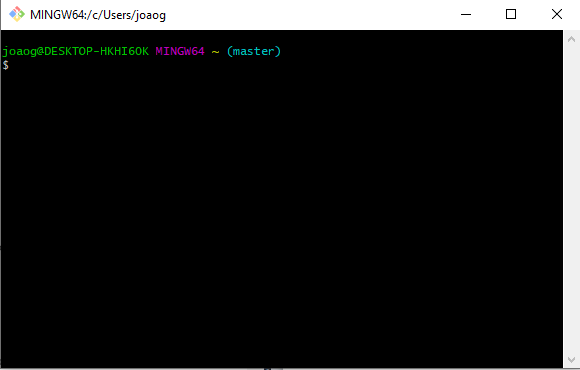
\includegraphics[width = 11cm]{images/gitBashInterface.png}  

Agora precisá-se entrar na pasta onde será definido o repositório local. Para isso, usa-se o comando do terminal \textit{cd "nome da pasta"} para acessar o caminho das pastas até onde será o local do repositório. Outra forma possível é ir ao local da pasta manualmente e clicar em abrir com \textit{Git Bash}.

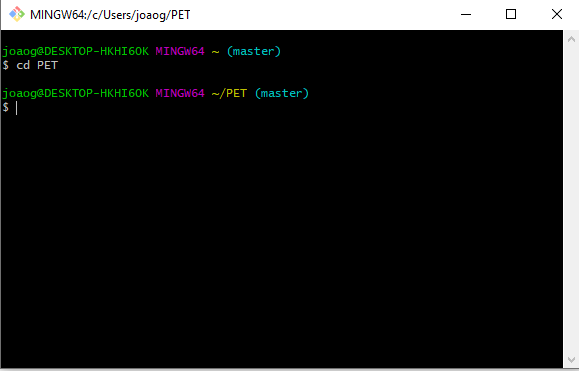
\includegraphics[width = 11cm]{images/cd.png}\\
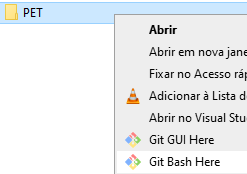
\includegraphics[width = 11cm]{images/abrirComBash.png}

Ao acessar o arquivo escolhido, deve-se iniciar o repositório local usando o comando \textit{git init} (FERNANDES, 2019)(1).

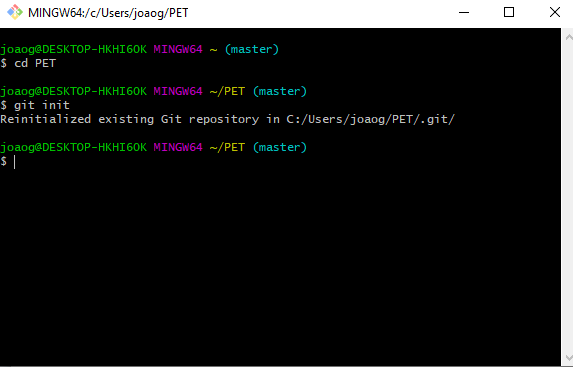
\includegraphics[width = 11cm]{images/gitInit.png}

Em seguida, verifica-se por mudanças na pasta que não foram enviadas para o repositório usando o \textit{git status}.

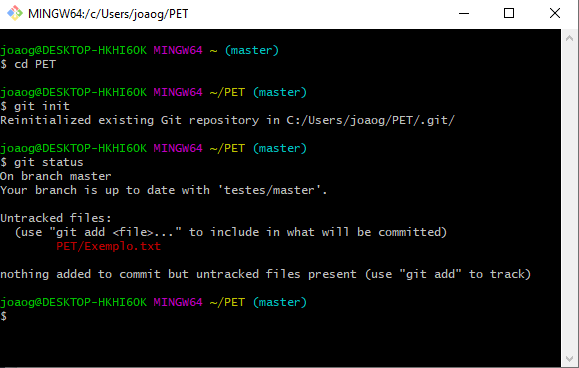
\includegraphics[width = 11cm]{images/gitStatus.png}

Ao verificar o status da pasta, deve-se adicionar os arquivos modificados na linha para o \textit{commit}. Existem duas formas de executar o comando: a primeira é colocar todas as mudanças da pasta de uma vez com o \textit{git add "pasta"} e a segunda colocar um arquivo por vez com o \textit{git add "arquivo"}.

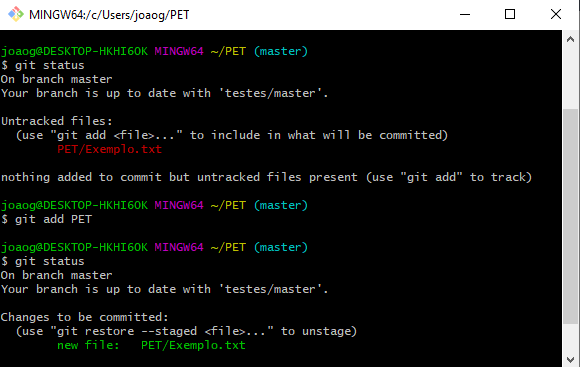
\includegraphics[width = 11cm]{images/gitAdd.png}

Depois de adicioná-los, pode-se passar para o repositório local com o comando \textit{git commit}. No caso desse comando é necessário mandar uma mensagem junto ao \textit{commit}. Para isso, é possível utilizar o comando \textit{git commit -m "mensagem a enviar"} ou colocar somente \textit{git commit}, o que te levará a outra tela onde deverá ser adicionada a mensagem e em seguida, selecionar \textit{"esc"} e digitar \textit{":wq"} para sair.

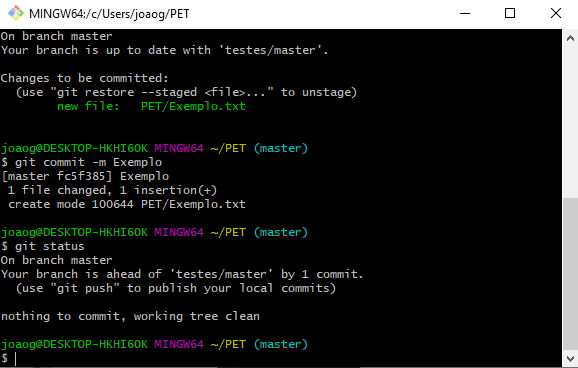
\includegraphics[width = 11cm]{images/gitCommit.png}

O próximo passo é mandar as mudanças para o repositório remoto. Para isso o seu \textit{Git} necessita estar conectado e configurado a algum repositório nas plataformas de hospedagem (ver a subseção 4.3 e 4.4). Depois de estar conectado, basta utilizar o comando \textit{git push -u origin "nome da branch que receberá os códigos"} para fazer o primeiro \textit{git push}. Nas próximas vezes que for usar o \textit{git push} é só escrever o comando \textit{git push} que ele mandará para a última \textit{branch} conectada, sem ter que escrever o comando inteiro.   

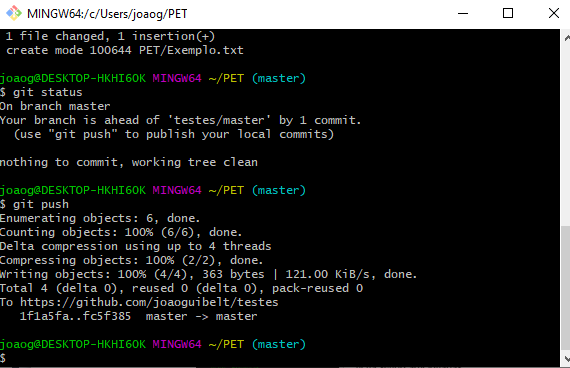
\includegraphics[width = 11cm]{images/push.png}

Com isso todas as mudanças feitas já foram guardadas no repositório remoto e foram versionadas, podendo ser acessadas a qualquer momento.

\subsubsection{Usando o \textit{Git} por uma interface gráfica}

\hspace{4mm}Além do terminal o \textit{Git} tem compatibilidade com uma variedade de interfaces gráficas como o \textit{sourcetree} e o \textit{GitKraken}, e até algumas interfaces específicas para certas plataformas de hospedagem como o \textit{GitHubDesktop}. Nelas o programador consegue de forma mais simples fazer os \textit{"commits"} e visualizar mais facilmente o que o \textit{Git} está fazendo, porém cada software desses funciona da uma forma diferente e tem suas vantagens e desvantagens que devem ser estudadas para o próprio programa.

\subsection{Conectando \textit{Git} com o \textit{GitHub}}

\hspace{4mm}Para que o programador consiga colocar os seus códigos no \textit{GitHub} pelo terminal ele precisa conectar o \textit{Git} ao seu repositório, para isso a forma mais simples é usando uma chave ssh (Tutorial completo e simples sobre a configuração de uma chave ssh no site do \textit{GitHub})(FERREIRA, 2015).

Com a chave configurada o programador precisa usar o comando \textit{git remote add origin "link do repositório"} para ligar o repositório ao \textit{Git} com o nome de \textit{origin} e assim ele terá total controle sobre o repositório.

\subsection{Trocando de \textit{branch}}
Outros comandos bem importantes são os que alteram as \textit{branchs}. Para criar uma nova \textit{branch} pelo \textit{Git} é só usar o comando \textit{git branch "nome da branch"} e para checar as \textit{branchs} ativas usar o comando \textit{git branch}. Quando as \textit{branchs} forem checadas aparecerá um asterisco do lado da que estiver sincronizada para receber os códigos, para trocar isso deve-se usar o comando \textit{git checkout "nome da branch a sincronizar"} que assim quando o programador fizer o \textit{git push} os \textit{commits} serão mandados para essa branch (FERNANDES, 2019)(2). 

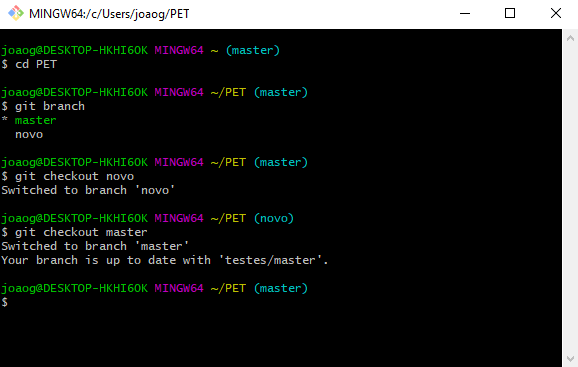
\includegraphics[width = 11cm]{images/branch.png}

Porém, para que uma nova \textit{branch} seja levada para o repositório remoto é necessário que ela seja permitida a fazer isso (o que se aplica para a \textit{branch} principal também). Para isso, na hora de usar o comando \textit{push} usa-se \textit{git push origin "nome da nova branch"}, assim, nas próximas vezes que for fazer o \textit{push} nessa \textit{branch} precisará somente usar o \textit{git push} (igual a \textit{branch} principal).  

\section{\textit{GitHub}}

\hspace{4mm}Outra parte importante de se conhecer é como unir as \textit{branchs} dentro do \textit{GitHub}. Quando executá-se o \textit{push} para uma \textit{branch} diferente da principal precisa-se checar as mudanças para depois fazer um \textit{"pull request"} para uni-las a principal. Isso acontece, pois, a ideia de ter \textit{branchs} diferentes é para que uma equipe de programadores consiga alterar o mesmo código sem que um interfira com o outro, facilitando muito projetos com grupos maiores. Para começar, quando as mudanças forem para o \textit{GitHub} a seguinte mensagem no repositório aparecerá. Sendo  "novo" o nome da \textit{branch}.


\includegraphics[width = 11cm]{images/gitHubPush.png}

Clicando no botão verde o site te levará para ver as mudanças e confirmar a união com a \textit{branch} principal.

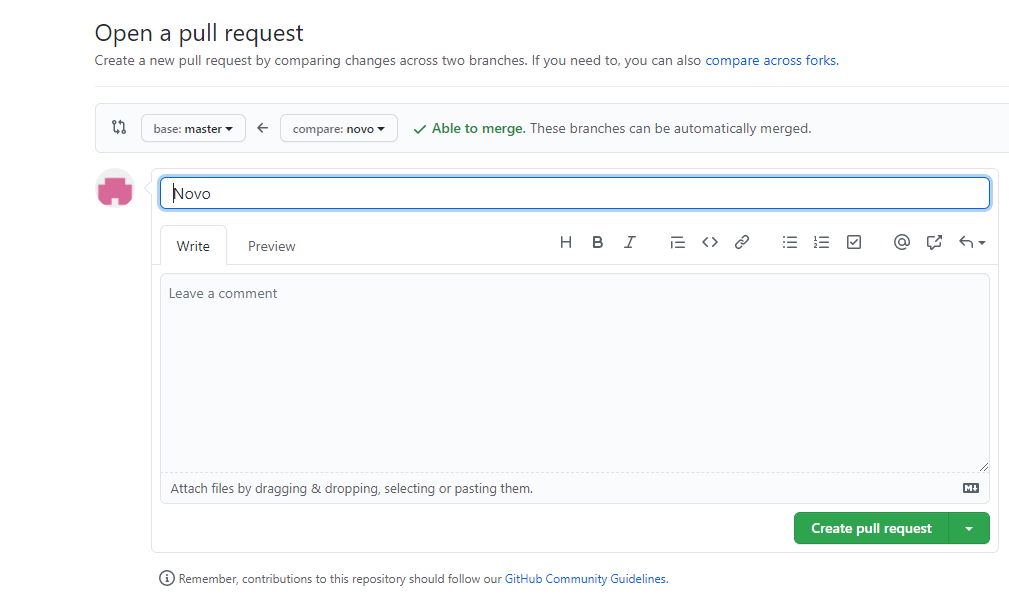
\includegraphics[width = 11cm]{images/pull.png}

Clicando em \textit{"create pull request"} e depois em \textit{"merge pull request"} na próxima página e confirmando, todos as mudanças da \textit{branch} serão mandadas para a \textit{branch} principal.

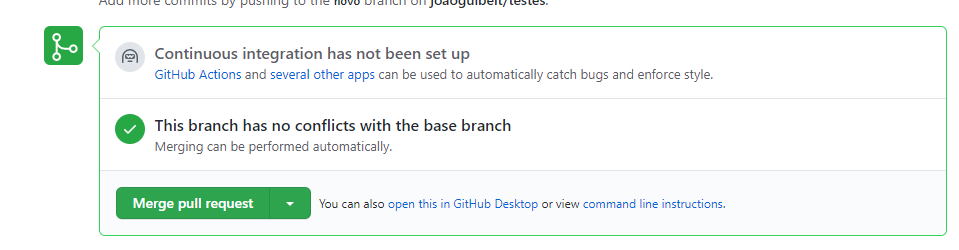
\includegraphics[width = 11cm]{images/merge.png}


\includegraphics[width = 11cm]{images/final.png}

Com isso feito o versionamento e armazenamento dos códigos foi feito com sucesso.

\section*{Conclusão}

\hspace{4mm}Concluindo, o uso de softwares de versão e plataformas de hospedagem de código-fonte como o \textit{git} e \textit{GitHub}, respectivamente, são essenciais para a organização e controle de projetos contemporâneos. Dessa forma, é sugerido o uso de tais software pelo grupo PET eu seus próximos projetos.

\section*{Refenrecias Bibliográficas}

[GUANABARA, 2020](GUANABARA, Gustavo. Curso grátis Git e Github. Youtube, 2020. Disponível em: https://www.youtube.com/watch?v=xEKo29OWILE&list\\=PLHz_AreHm4dm7ZULPAmadvNhH6vk9oNZA. Acesso em: 13mar2021).

[BERTOLA, 2019](BERTOLA, Fernanda. Git, Github e Gitlab: o que são e principais diferenças. \textbf{Zup}, 2019. Disponível em: https://www.zup.com.br/blog/git-github-e-gitlab. Acesso em: 14mar2021).

[FERNANDES, 2019](1)(FERNANDES, Maurício. Git na prática — Parte 1 (Subindo projeto para o github).\textbf{Medium}, 2019. Disponível em: https://medium.com/nstech/git-e-github-por-que-e-como-usar-parte-2-d00c3b248822. Acesso em: 15mar2021).

[FERREIRA, 2015](FERREIRA, Gabs. Instalando o Git e configurando Github no Windows. \textbf{Gabsferreira},2015. Disponível em: http://gabsferreira.com/instalando-o-git-e-configurando-github/. Acesso em: 14mar2021).

[FERNANDES, 2019](2)(FERNANDES, Maurício. Git e Github — Por que e como usar? — Parte 2.
\textbf{Medium}, 2019. Disponível em: https://medium.com/nstech/git-e-github-por-que-e-como-usar-parte-2-d00c3b248822. Acesso em: 15mar2021).


\section*{Exemplo}

Exemplo de commit.

\end{document}
